\documentclass[10pt,a4paper]{article}
\usepackage[utf8]{inputenc}
\usepackage{amsmath}
\usepackage{amsfonts}
\usepackage{amssymb}
\usepackage[hidelinks]{hyperref}
\usepackage{cleveref}
\usepackage{tikz}
\usepackage{listings}
\usepackage{float}
\usepackage[cache=false]{minted}
% Make clickable footnote
\newcommand{\hyperfootnote}[1][]{\def\ArgI\hyperfootnoteRelay}
% relay to new command to make extra optional command possible
\newcommand\hyperfootnoteRelay[2][]{\href{#1#2}{\ArgI}\footnote{\href{#1#2}{#2}}}
\usepackage{fullpage}
\author{Saran Ahluwalia and Mountain Chan}
\title{Implementation of the 2-D Solution for the Poisson Equation on the Dirichlet Boundary}

\newcommand{\crefrangeconjunction}{--}

\usepackage{color} %red, green, blue, yellow, cyan, magenta, black, white
\definecolor{mygreen}{RGB}{28,172,0} % color values Red, Green, Blue
\definecolor{mylilas}{RGB}{170,55,241}

\makeatletter
\DeclareTextCommand{\textprime}{\encodingdefault}{%
  \mbox{$\m@th'\kern-\scriptspace$}% 
}
\makeatother

\begin{document}
\maketitle

\lstset{language=python,%
    %basicstyle=\color{red},
    breaklines=true,%
    morekeywords={matlab2tikz},
    keywordstyle=\color{blue},%
    morekeywords=[2]{1}, keywordstyle=[2]{\color{black}},
    identifierstyle=\color{black},%
    stringstyle=\color{mylilas},
    commentstyle=\color{mygreen},%
    showstringspaces=false,%without this there will be a symbol in the places where there is a space
    numbers=left,%
    numberstyle={\small \color{gray}},% size of the numbers
    numbersep=9pt, % this defines how far the numbers are from the text
    emph=[1]{for,end,break},emphstyle=[1]\color{red}, %some words to emphasise
    %emph=[2]{word1,word2}, emphstyle=[2]{style},    
}


\section*{Introduction}
The Dirichlet boundary value problem is a variant of the boundary value problem in which the function on the boundary is as follows:
\begin{subequations}
  \begin{align}
  \hat{\mathcal{S}} u(x_1 , ... , x_n) &= f(x_1 , ... , x_n) \label{eqn: dirichlet 1}\\
  u(x_1, ..., x_n) &= g(x_1, ..., x_n) \,\, \text{for} \,\, \forall (x_1, ..., x_n) \in \partial\Omega \label{eqn: dirichlet 2}
  \end{align}
\end{subequations}

where $\hat{\mathcal{S}}$ is a linear differential operator consisting of the summand of any order derivative including heterogenuous partial derivatives. Moreover, $u$, $f$, and $g$ are functions of $n$ variables from $\mathbb{R}^n$ to $\mathbb{R}$. The problem is solved on a domain $\Omega \subset \mathbb{R}^n$ with a defined boundary $\partial \Omega$. In essence, the Dirichlet problem is a boundary value problem in which the solution value is a function. This is diametrically opposed to the Neumann problem in which the value of the solution's derivative is on the boundary \footnote{Greenspan, Donald. “Numerical Analysis and the Dirichlet Problem.” Mathematics Magazine, vol. 32, no. 4, 1959, pp. 177–188. JSTOR, www.jstor.org/stable/3029112.}.

The Dirichlet problem is very useful in a variety of fields. In particular, differential equations that are often used with Dirichlet boundary conditions include the  Laplace equation, Poisson equation and diffusion. The aforementioned are actually all more general forms of the Laplace equation; the Poisson equation is a non-homogeneous form while the diffusion equation adds first and second derivative terms, respectively \footnote{Volker John's Course Notes for PDE and numerical analysis: \url{https://www.wias-berlin.de/people/john/LEHRE/NUM_PDE_FUB/num_pde_fub.pdf}}.

The Laplace equation

\begin{equation}
\Delta u = 0 \label{eqn: laplace}
\end{equation}

is a partial differential equation used with Dirichlet boundary conditions. The solutions to this equations are harmonic functions. On the other hand, the Laplace equation is leveraged in machine learning. In particular, there is an emerging interest in its exploitation in natural language processing within the context of reducing dimensions for vectorized word embeddings. Moreover, this operator is often used to smooth the gradient during batch gradient descent \footnote{Stanford CS229: Machine Learning: \url{http://cs229.stanford.edu/notes/cs229-notes1.pdf} }.
The Poisson equation

\begin{equation}
\Delta u = f \label{eqn: poisson}
\end{equation}

is the non-homogeneous form of \cref{eqn: laplace}. The Poisson equation representation for $f$ can be used to represent forces such as gravity, electromagnetism, and fluid forces. Recent developments in its application are also in neural networks in order to solve elliptic PDEs. A network is constructed for the boundary and another for the PDE network. Here an update on the boundary occurs multiple times before a single evaluation on the interior. Thereafter, the loss function is a computed based off of the boundary loss and interior loss\footnote{Deep Learning for PDEs: \url{http://stanford.edu/~kailaix/files/Deep_Learning_for_Partial_Differential_Equations.pdf}}. In the former applications, $u$ represents a potential, which can be related to a force via Newton's second law or can be used in energy analysis. The $f$ term comes from a source origin. In the case of an electrostatic field, we have $f = - \frac{\rho (r)}{\epsilon_0}$, where $\rho$ is the radial charge density; the gravitational source term is $f = 4 \pi^2 G \rho(r)$, where $G$ is the universal gravitational constant and $\rho$ is the radial mass density\footnote{Lecture Notes by Anthony Pierce: Solving the Heat, Laplace and Wave equations using finite difference methods \url{https://www.math.ubc.ca/~peirce/M257_316_2012_Lecture_8.pdf.}}.


In the latter applications, there have been novel approaches that reliably compute many useful properties of a silhouette for images. It has been previously been show that this function can be used to reliably extract various shape properties including part structure and rough
skeleton, local orientation and aspect ratio of different parts, and convex and concave sections of the boundaries. This abets in shape classification algorithms \footnote{Shape Representation and Classification Using the Poisson Equation \url{http://www.wisdom.weizmann.ac.il/~meirav/TPAMI-0429-0805-1.pdf}.}.

\section*{Mathematical Theory}
There are myriad methods to solve \cref{eqn: laplace}. Analytically, this equation is often solved through the separation of variables. Specifically, with Dirichlet boundary conditions, the Lapace equation may be solved by using Green's function; however, both of these aforementioned techniques can become infeasible depending on the domain on which the problem is being solved. Hence an exploration utilizing numerical methods is warranted in order to provide a more exhaustive heuristic to solve these equations.

While numerical methods do not necessarily yield a solution in terms of analytic functions, they do provide abstract depictions of the solution. The solution and parameters can be adjusted in order to minimize error within a certain threshold. Additionally, once written, numerical methods can be used on a variety of variations of the problem and are often solved more expeditiously. Numerical data can even be fitted by functions to make approximations of analytic solutions.

Numerical solutions represent discrete relations rather than continuous ones and can be formulated by transforming the differential equation into a linear system. In this case, we have Poisson's equation with a Dirichlet boundary on a domain $\Omega \subset \mathbb{R}^2$

\begin{subequations}
  \begin{align}
  -u_{xx} - u_{yy} &= f(x, y) & \\
  u(x, y) &= 0 \,\, \text{for} \,\, \forall(x, y) \in \partial \Omega
  \end{align}
\end{subequations}

The domain $\Omega$ is depicted in \cref{fig: domain}. The domain could be scaled to arbitrary sizes; however, it is more feasible to utilize $\Omega$ to be unit squares.

\begin{figure}[H]
\center
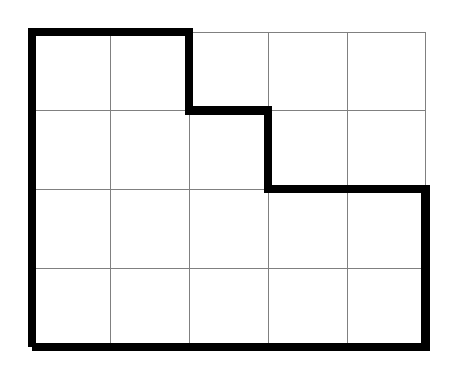
\begin{tikzpicture}
\draw[help lines] (0,0) grid (5,4);
\draw[line width=3] (0,0) -- (5,0) -- (5,2) -- (3,2) -- (3,3) -- (2,3) -- (2,4) -- (0,4) -- (0,0);
\end{tikzpicture}
\caption{Domain $\Omega$}
\label{fig: domain}
\end{figure}

To solve a differential equation numerically, we must discretize the differential operator into steps. A starting point for this is the limit definition of a derivative \footnote{From Vivi Andasari 2015 Course \url{http://people.bu.edu/andasari/courses/Fall2015/be503703Fall2015.html}.}

\begin{equation}
\label{eqn: limit derivative}
f'(a) = \lim\limits_{h \to 0} \frac{f(a + h) - f(a)}{h}
\end{equation}

To discretize this limit we allow $h \to \Delta h$, where $\Delta h$ is minimal and decreases in order to improve the accuracy of the result. This relation can be used with a Taylor series to find relations for higher-order derivatives (as Dr.Moody Chu discussed in lecture). Applying this to find the Laplace operator for $\mathbb{R}^2$ and indexing values yields the algebraic relation

\begin{equation}
\label{eqn: laplacian algebra}
- \Delta u(x_i, y_j) = \frac{4u_{ij} - u_{i+1, j} - u_{i+1, j} - u_{i, j+1} - u_{i, j-1}}{\left( \Delta h \right)^2}
\end{equation}

With \cref{eqn: laplacian algebra}, an operator matrix $\hat{A}$ may be formed such that $\hat{A} \vec{u}$ is a discretized form of $\Delta u$ for $\vec{u}$ is a vector formed by $u(x_i, y_j)$, where $x_i$ and $y_j$ are  points that are created when the boundary $\Omega$ is separated into a mesh with step size $\Delta h$. We then obtain a linear system

\begin{equation}
\label{eqn: linear system}
\hat{A} \vec{u} = \vec{f}
\end{equation}

where $\vec{f}$ is the vector created from $f(x_i, y_j)$ evaluated at the same mesh points as $\vec{u}$. 

This system can be solved by several different methods. To simplify the computation, the $\Delta h$ term is factored out of $\hat{A}$ and placed with the function term

\begin{equation}
\label{eqn: linear system 2}
\hat{A}\textprime{} \vec{u}  = \left( \Delta h \right)^2 \vec{f}
\end{equation}

 where $\hat{A}\textprime{} \equiv \left( \Delta h \right)^{-2} \hat{A}$. With this system defined by the operator in \cref{eqn: laplacian algebra}, we have an error of order $\left( \Delta h \right)^4$  \footnote{From Dr. Robert Hunt's Course at Cambridge University \url{http://www.damtp.cam.ac.uk/user/reh10/lectures/nst-mmii-chapter2.pdf}.}. 

 \section*{Computational Details}
 
Below is detailed part 1(a) of this assignment which entailed depicting the operator matrix with the $7 \times 7$ dimension $A$ in a table format:
$$\begin{tabular}{|l|l|l|l|l|l|l|}
\hline
% U(1,1) & U(2,1) & U(3,1) & U(4,1) & U(1,2) & U(2,2) & U(1,3) \\ \hline
4      & -1     & 0      & 0      & -1     & 0      & 0      \\ \hline
-1     & 4      & -1     & 0      & 0      & -1     & 0      \\ \hline
0      & -1     & 4      & -1     & 0      & 0      & 0      \\ \hline
0      & 0      & -1     & 4      & 0      & 0      & 0      \\ \hline
0      & 0      & 0      & 0      & 4      & -1     & -1     \\ \hline
0      & 0      & 0      & 0      & -1     & 4      & 0      \\ \hline
0      & 0      & 0      & 0      & -1     & 0      & 4      \\ \hline
\end{tabular}$$ 

 
Programmatically, in order to solve this problem, Python 3.6, with packages NumPy, SciPy and Matplotlib was used. Prototyping and validation of the generic solver and the solutions for (1a) and (1b) were performed leveraging Matlab in order to verify dimension structure and adherence to project-specific requirements. Specifically, the validation was isolated to the construction of the operator matrix, the augmented domain and solution vectors. Subsequently these evaluations were computed with SciPy, transformed into the Matlab API for full double arrays and then plotted using the surf API \footnote{Mathworks Surf Plotting \url{https://www.mathworks.com/help/matlab/ref/surf.html}}. Relevant Python snippets are displayed in this section.

Briefly, the first step for solving a given problem is to establish a domain matrix. Subsequently, the step size is used to construct a mesh grid  which is $\Delta h$ in \cref{eqn: laplacian algebra}. Programmatically a matrix was furnished in order to represent the interior points within the domain. For example, the matrix that represents the domain of interest shown in \cref{fig: domain} is given by. This is the base domain that was provided for problem one. This domain was subsequently extrapolated to a generic solution for part two.

\begin{displaymath}
\left[
\begin{matrix}
1 & 0 & 0 & 0 \\
1 & 1 & 0 & 0 \\
1 & 1 & 1 & 1 
\end{matrix}
\right]
\end{displaymath}

This matrix that can be any matrix in $ \mathbb{R}^{m \times n}$ represents $m$ the maximum $y$ value of the domain and $n$ and where the maximum $x$ value of the domain if the domain is split into unit squares. A $1$ represents a unit square while a $0$ represents a location in space that is not in the domain. This heuristic enables any solver to extrapolate the solution matrix to any arbitrary domain. Hence, this matrix can be of any dimension and the dimension can be scaled to more accurately represent nonlinear features.

 Furthermore, splitting the domain via the unit squares of the domain entails repeating $\frac{1}{\Delta h}$ times in both their column and the next row. For example, when a step size of $\Delta h = \frac{1}{2}$ is used, the aforementioned matrix undergoes the transformation

\begin{displaymath}
\left[
\begin{matrix}
1 & 0 & 0 & 0 \\
1 & 1 & 0 & 0 \\
1 & 1 & 1 & 1 
\end{matrix}
\right]
\to
\left[
\begin{matrix}
	1 & 1 & 1 & 0 & 0 & 0 & 0 & 0 & 0\\
	1 & 1 & 1 & 0 & 0 & 0 & 0 & 0 & 0\\
	1 & 1 & 1 & 1 & 1 & 0 & 0 & 0 & 0\\
	1 & 1 & 1 & 1 & 1 & 0 & 0 & 0 & 0\\
	1 & 1 & 1 & 1 & 1 & 1 & 1 & 1 & 1\\
	1 & 1 & 1 & 1 & 1 & 1 & 1 & 1 & 1\\
	1 & 1 & 1 & 1 & 1 & 1 & 1 & 1 & 1
\end{matrix}
\right]
\end{displaymath}

Thus, empirical evidence suggests a delta value of $\Delta h \leq 1$ is optimal and empirically appears to produce the most refined solutions. Empirically, we confirmed that smaller $\Delta h$ sizes improved solutions, controlling for the domain and function. Unfortunately, due to time constraints and task prioritization accrued results of the runtime are not presented in this section.  

The Kronecker product\footnote{Mathworks Documentation for Kronecker product: \url{https://www.mathworks.com/help/matlab/ref/kron.html}.} was used in order to expand the rows and columns by the step size. Subsequently, a row and column are concatenated, vertically and horizontally along the dimension in order to normalize the missing interior points in both the domain of $x$ and $y$.

The aforementioned procedure for creating the \cref{eqn: linear system 2} is relatively fast, even with relatively large ($k$ dimensional) matrices. Specifically, in Python for a step size of 32, the mean time for this step was 0.009035 seconds with the following operating system specifications: 2 vCPU @ 2.2GHz and 13GB RAM. This is not surprising considering that NumPy arrays and matrices are written in C.


The next step for the algorithm is to construct the actual operator matrix $\tilde{\hat{A}}$. Due to the $4u_{ij}$ term in \cref{eqn: laplacian algebra}, it was proven in class that the diagonals of $\tilde{\hat{A}}$ are 4. Thus initializing an identity matrix is created and multiplied by the scalar, four. For a given point in the domain, the interior points are found by finding points in the expanded domain with a combination of both NumPy's \textbf{nonzero} and \textbf{where} functions and interrogating the immediate neighbors, above, below, left, and right, of the given point.

% \lstinputlisting[language=Matlab, firstline=24, lastline=53, firstnumber=24]{centralDifferencePoisson.m}


The interior structure of the matrix can be seen using Matplotlib's axes library's \textbf{spy} command and resulted in the figure below \cref{fig: operator matrix}. The figure below indicates that the matrix is sparse. We leveraged SciPy's CSR formatted sparse matrix \footnote{SciPy CSR Sparse Matrix Documentation \url{https://docs.scipy.org/doc/scipy/reference/generated/scipy.sparse.csr_matrix.html}.} for the generic solver in order to compute more performant solutions for smaller step sizes.

For example, with a step size of $h = \frac{1}{1028}$ (run on Google Compute (GCE) \footnote{Google Compute Engine \url{https://cloud.google.com/compute/}}  standard machine type with 8 vCPUs and 30 GB of memory) reduced memory usage, on average, from approximately $20000$MB to approximately $4000$MB after 10 trials. 

\begin{figure}[H]
\center
\includegraphics[scale=0.3]{figures/operator-spy.eps}
\caption{Operator Matrix Structure}
\label{fig: operator matrix}
\end{figure}


\begin{figure}[H]
\includegraphics[width=\linewidth]{figures/rows_first.png}
\includegraphics[width=\linewidth]{figures/rows_last.png}
\caption{ 43 x 43 Operator Matrix for domain $\omega$ }
\label{fig: pdetool gaussian solutions}
\end{figure}

\begin{figure}[H]
\center
\includegraphics[scale=0.3]{figures/p1b_diagonal.png}
\caption{Operator Matrix Spy for 43 X 43}
\label{fig: operator matrix}
\end{figure}

Finally, the right hand side solution vector is constructed before solving the linear system with NumPy's linear algebra module for solving the right-hand side of \cref{eqn: linear system 2}. This is performed by evaluating each $f(x,y)$ at each of the  points in the domain, embedding the result in the resulting array and applying the product with $\left( \Delta h \right)^2$. Subsequently the linear system is solved.

In addition to solving the system, the generic solver throws out all $x$ and $y$ coordinates that are not in the domain. This part of the algorithm is needed in order to properly visualize all solutions within the constraints of the surface's domain.

\subsection*{Python Code}

\subsubsection{Part 1a}

 
\inputminted{python}{code/part_one_solver.py}


\subsubsection{Part 1b}

 
\inputminted{python}{code/problem_one_part_two.py}


\subsubsection{Generic Solver}

 
\inputminted{python}{code/matrix_solver.py}

 \section*{Conclusion}
 
\begin{subequations}
\begin{align}
f(x, y) =& x e^{-x^2 - y^2} \label{eqn: gaussian}\\
f(x, y) =& x \left( x - y \right)^3 \label{eqn: cubic}
\end{align}
\end{subequations}

The generic solver, above, was used to solve the Gaussian and cubic functions, \cref{eqn: gaussian} and \cref{eqn: cubic}, respectively. Due to local OS limitations, conflated with prevarication of heap memory by resource intensive applications such as the Chromium driver, we were limited to solving the solution with a solution of $\Delta h = \frac{1}{32}$ for \cref{eqn: gaussian} and $\Delta h = \frac{1}{64}$ for \cref{eqn: cubic}, respectively. The solution plots were compared with the solutions found by Matlab's built-in PDE toolbox\footnote{Mathworks PDE Toolbox \url{https://www.mathworks.com/products/pde.html}}. These plots are shown in \crefrange{fig: gaussian solutions}{fig: pdetool cubic solutions} (below). The plots in \cref{fig: steps} display the evolving solution for step sizes for  $1, 2, 4, 8$ and the precipitous convergence to the solution.

The generic solver is able to handle any arbitrary domain in the current implementation. This flexibility makes it ideal for solving more complex problems over myriad domains. However, it should be noted that the solutions for the given step sizes are markedly worst than the PDE-Toolbox's solver, and due to it's iterative implementation is extremely expensive and inefficient. In fact the current algorithm's implementation is at worst quadratic running time, $\mathcal{O}(n^2)$ where n is the number of interior points within the $x-$axis domain.

To account for this, a more complex functional data structure, such as a ConcTree \footnote{Conc-Trees for Functional and Parallel
Programming \url{http://aleksandar-prokopec.com/resources/docs/lcpc-conc-trees.pdf}}. This would allow for the domain into several subsets that can be evaluated upon using separate processes and then joined upon convergence. Another variant is to utilize Voronoi partitions in order to sub-divide the domain into more discrete points and then seek neighbors using k-nearest neighbors. These are of course optimizations on the representation of the domain.

Finally, another variant, specific to kinetic motion, would be an implementation of a the parallel Barnes-Hut algorithm for $N$-body simulation. $N$-body simulation is a simulation of a system of $N$ particles that interact with physical forces, such as gravity or electrostatic force. Given initial positions and velocities of all the particles (or bodies), the $N$-body simulation computes the new positions and velocities of the particles as the time progresses. It does so by dividing time into discrete short intervals, and computing the positions of the particles after each interval.

To take advantage of this observation, the Barnes-Hut algorithm relies on a quadtree -- a data structure that divides the space into cells, and answers queries such as 'What is the total mass and the center of mass of all the particles in this cell?'

An iteration of the Barnes-Hut algorithm is composed of the following steps:

\begin{description}
  \item[$\bullet$ 1] Construct the quadtree for the current arrangement of the bodies.
  \item[$\bullet$ 2] Determine the boundaries, i.e. the square into which all bodies fit.
  \item[$\bullet$ 2] Construct a quadtree that covers the boundaries and contains all the bodies.
\end{description}
Then, 
    (i) Update the bodies -- for each body:
    (ii) Update the body position according to its current velocity.
    (iii) Using the quadtree, compute the net force on the body by adding the individual forces from all the other bodies.
    (iv) Update the velocity according to the net force on that body.
    
It turns out that, for most spatial distribution of bodies, the expected number of cells that contribute to the net force on a body is $log(n)$. Hence the overall complexity of the Barnes-Hut algorithm is  $\mathcal{O}(n\log{}n)$! 

In conclusion, this exercise affords many new avenues to solve this problem; this brief synopsis provides a solid foundation in order to further explore computational complexity within higher dimensional spaces and non-linear problems. 

\pagebreak
\subsection*{Solutions}


\begin{figure}[H]
\includegraphics[width=0.5\linewidth]{figures/part1aside.png}
\includegraphics[width=0.5\linewidth]{figures/part1atop.png}
\includegraphics[width=0.5\linewidth]{figures/part1bside.png}
\includegraphics[width=0.5\linewidth]{figures/part1btop.png}
\caption{Solutions to Part 1a with step size of 1 (top) and 1b with step size of 1/2 (bottom), respectively}
\label{fig: steps}
\end{figure}




\begin{figure}[H]
\includegraphics[width=0.5\linewidth]{figures/gaussian-h1.png}
\includegraphics[width=0.5\linewidth]{figures/gaussian-h2.png}
\includegraphics[width=0.5\linewidth]{figures/gaussian-h4.png}
\includegraphics[width=0.5\linewidth]{figures/gaussian-h8.png}
\caption{Solutions to \cref{eqn: gaussian} with $\Delta h = 1, 2, 4, 8 $ and $32$ (below). Color palette adjusted in order to highlight contrast in value approximations at each cell in the domain}
\label{fig: steps}
\end{figure}

\begin{figure}[H]
\includegraphics[width=\linewidth]{figures/gaussian-64-top.eps}
\includegraphics[width=\linewidth]{figures/gaussian-64.eps}
\caption{Solutions to \Cref{eqn: gaussian}}
\label{fig: gaussian solutions}
\end{figure}


\begin{figure}[H]
\includegraphics[width=0.5\linewidth]{figures/eqTwosizeOne.png}
\includegraphics[width=0.5\linewidth]{figures/eqTwosizeHalf.png}
\includegraphics[width=0.5\linewidth]{figures/eqTwosizeQuarter.png}
\includegraphics[width=0.5\linewidth]{figures/eqTwosizeEighth.png}
\caption{Solutions to \cref{eqn: cubic} with $\Delta h = 1, 2, 4, 8$}
\label{fig: steps}
\end{figure}


\begin{figure}[H]
\includegraphics[width=\linewidth]{figures/gaussian-top-pdetool.png}
\includegraphics[width=\linewidth]{figures/gaussian-iso-pdetool.png}
\caption{PDE Toolbox Solutions to \Cref{eqn: gaussian}}
\label{fig: pdetool gaussian solutions}
\end{figure}

% \begin{figure}[H]
% \includegraphics[width=\linewidth]{figures/cubic-64-top.eps}
% \includegraphics[width=\linewidth]{figures/cubic-64.eps}
% \caption{Solutions to \Cref{eqn: cubic}}
% \label{fig: cubic solutions}
% \end{figure}

\begin{figure}[H]
\includegraphics[width=\linewidth]{figures/cubic-top-pdetool.png}
\includegraphics[width=\linewidth]{figures/cubic-iso-pdetool.png}
\caption{PDE Toolbox Solutions to \Cref{eqn: cubic}}
\label{fig: pdetool cubic solutions}
\end{figure}




\end{document}
